\documentclass[11pt]{article}
\usepackage[utf8]{inputenc}

\title{Recipe Recommendations}
\author{Easton Potokar}
\date{March 2020}

\usepackage{graphicx}
\usepackage{hyperref}
\usepackage{natbib}
\usepackage{amsmath}
\usepackage{xcolor}
\usepackage[margin=1.5in]{geometry}

\newcommand\todo[1]{\textcolor{red}{TODO: #1 \\}}
% \renewcommand\todo[1]{}

\newcommand*\textfrac[2]{
  \frac{\text{#1}}{\text{#2}}
}

\begin{document}

\maketitle

\begin{abstract}
    We seek to explore making a personalized recipe recommendation system based on ingredients, tags, and past user reviews. We analyze both the accuracy of the recommendations as well as the temporal complexity of making them. We find that we can make very accurate recommendations to satisfy what cravings people may have and those they didn't know they had.
\end{abstract}

\section{Problem Statement and Motivation}
Machine Learning algorithms that make recommendations to users are becoming more and more common and are seen all over the internet for movies, friends, web searches, etc. A less common application is that of recipe suggestions. Is it possible to find a perfect recipe for someone given their past preferences of foods? Or a recommendation based on what their current cravings and pantry look like? 

\todo{More research on what's been already done.}


\section{Data}
\begin{figure}[t]
\centering
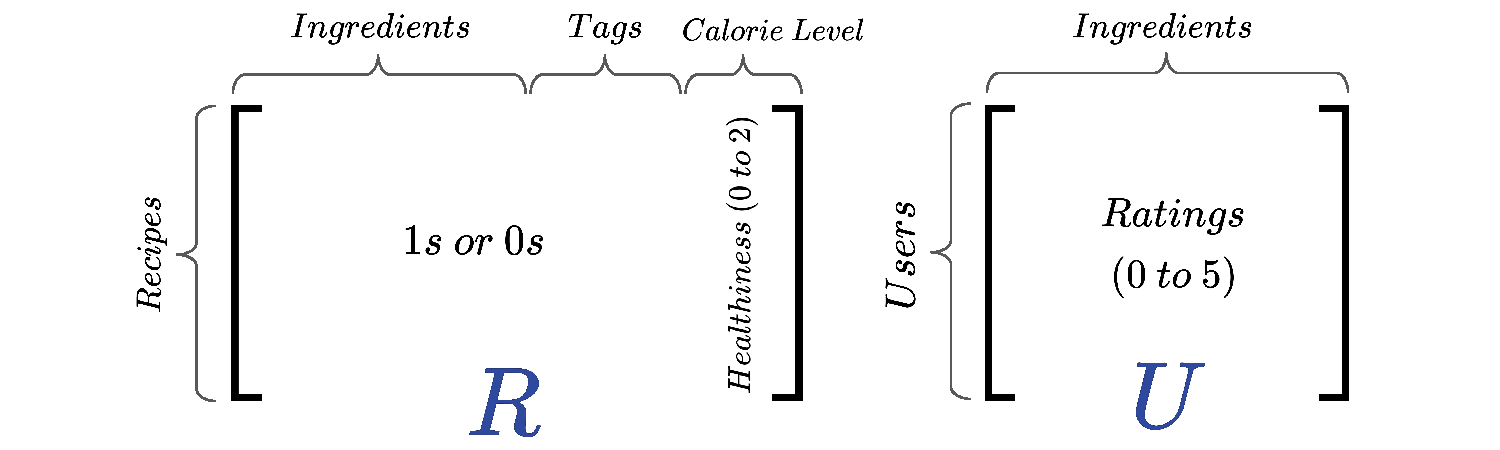
\includegraphics[width=0.9\textwidth]{figs/data.pdf}
\caption{Data Overview}
\label{fig:data_overview}
\end{figure}

Our data was gathered from \cite{data}, whose dataset can be found at \href{https://www.kaggle.com/shuyangli94/food-com-recipes-and-user-interactions}{here}. The data consists of more than 180 thousand recipes (made up of their ingredients, calorie level, and various tags describing them), and 700 thousand user reviews of the 180 thousand recipes all scraped from Food.com  and ranging from 0 to 5 stars. The original authors of the data used various natural language processing techniques to parse the recipes into about 8 thousand unique ingredients, around 500 unique tags, and a calorie level that is a 0, 1, or 2 denoting low-calorie to high-calorie recipes. To visualize what we're saying here see Figure \ref{fig:data_overview}.

The data appears to be very reliable, having been scraped directly from Food.com with the scraper being publicly available on github \cite{data_scraper}. Furthermore, it was used in a published research article, so one would hope everything was done ethically and correctly. The dataset is plenty large enough to give use meaningful answers to our questions and should be able to make a fairly robust recommendation system.


\section{Ethical Ramifications}
As with all recommendation systems, we must be careful what sort of bias we program into our algorithms. It would be very easily to heavily weight the algorithms to favor low-calorie recipes (healthier options) in an effort to push the public towards eating more healthy. While this would likely be well intentioned, in a way it is removing one's freedom of options, and is manipulating user's behaviors. Many similar biases must also be carefully considered, whether it be toward a certain ingredient/brand (company sponsorship), a certain ethnic preference (potentially racist), etc.

\section{Methods}

\subsection{Data Preparation}
\begin{figure}[t]
\centering
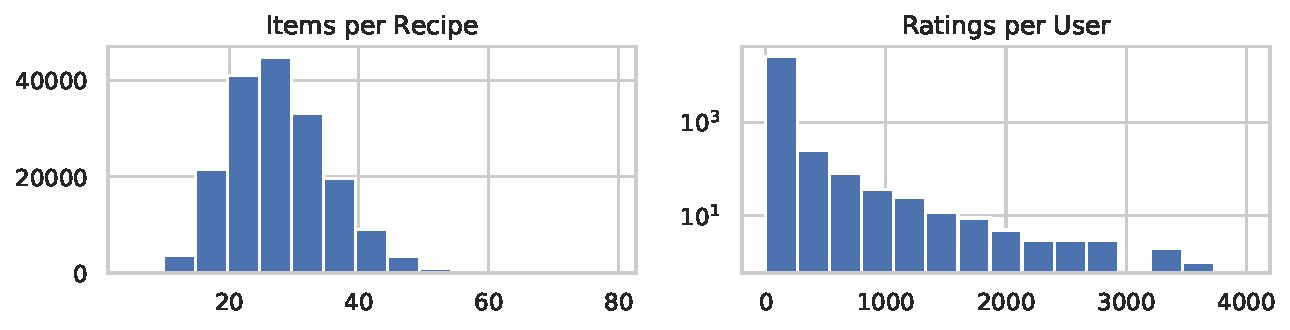
\includegraphics[width=0.9\textwidth]{figs/dist.pdf}
\caption{Data Overview}
\label{fig:dist}
\end{figure}

Note our data is on the format as seen in \ref{fig:data_overview}. This is a far from perfect solution. Note that the importance of a recipe having salt will be just as important as a recipe having jasmine or a jalapeno pepper. Commonly used in document classification, we use "TF-IDF" to help with this problem. In our case, we change each entry using the conversion (where item means either ingredient/tag):

$$\textfrac{\# of $i$th item}{Total \# of items in Recipe} * \log \Big( \textfrac{Total \# of Recipes}{\# of Recipes with $i$th item} \Big)$$

We perform the same transformation on the user dataset, replacing item with rating, and recipes with users. Throughout this document we analyze our data in both forms in order to visualize which data helps the algorithms perform the best.

To give ourselves a little intuition, we also visualize the distributions of how many items a recipe has and how many recipes a user has rated. This can be seen in Figure \ref{fig:dist}.


\subsection{Recommendation Process}
Most recommendation systems or "filtering" systems are considered either content-based or collaborative-based filtering. Content based systems make recommendations on attributes of the items; in our case this would be ingredients and tags of our recipes. Collaborative-based filtering uses the history of other users who are similar to us to recommend items. We'll explore using both. Our workflows will be as shown in Figure \ref{fig:flow}.

\begin{figure}[t]
\centering
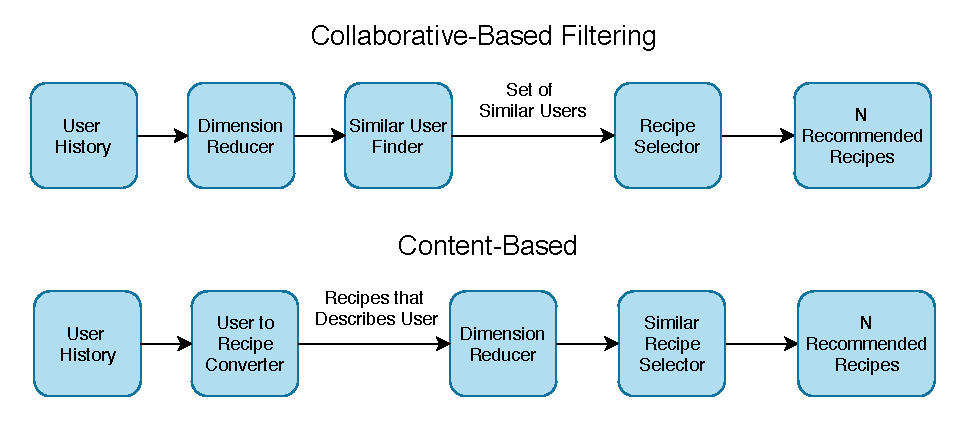
\includegraphics[width=1\textwidth]{figs/flow.pdf}
\caption{Recommendation Systems Flow}
\label{fig:flow}
\end{figure}

\subsubsection{Collaborative-Based Filtering}
We'll go over what was attempted in each step of collaborative-based filtering
\begin{enumerate}
    \item \textbf{Dimension Reducer}. PCA, LDA, NMF and Kernelized PCA were all used. Probablistic PCA and Sparse PCA were also attempted, but don't play well with sparse input. Kernelized PCA was also too computationally expensive and often abandoned.
    \item \textbf{User Finder}. We tried various algorithms for this:
    \begin{itemize}
        \item k Nearest Neighbor (kNN).
        \item Various Clustering Algorithms. Return all other users found in same cluster. Attempted using KMeans, GMM, MinCut, and DBSCAN.
        \item Combination of clustering and kNN. Return k nearest neighbors found in cluster. Could be more computationally effective.
    \end{itemize}
    We also take care to make sure our user finder doesn't return the input user.
    \item \textbf{Recipe Selector}. Taking the users passed to it, count number of times recipes are rated by user set along with their rating. Choose from among recipes by:
    \begin{itemize}
        \item Sorting by sum of ratings and return largest N sums
        \item Sorting by frequency and then by average rating. Return N largest.
        \item Sorting by average rating and then frequency.Return N largest.
    \end{itemize}
\end{enumerate}

\subsubsection{Content-Based Filtering}
We'll go over what was attempted in each step of content-based filtering
\begin{enumerate}
    \item \textbf{User to Recipe Converter}. We attempt this in two ways:
    \begin{itemize}
        \item Take all recipes with rating from user above a threshold. This method keeps each recipe separate (SR).
        \item Take all ingredients from recipes with rating from user above a threshold and combine into one huge recipe. (TR) 
    \end{itemize}
    \item \textbf{Dimension Reducer}. Dimensions were reduced in the same way as in the Collaborative-Based Approach.
    \item \textbf{Similar Recipe Selector}. In the case where the set of user describing recipes is a singleton, simply take the N NNs. In the case it isn't, take k NNs of each recipe and return the N most frequent.
\end{enumerate}

\subsubsection{Scoring}

To evaluate our models, we removed around 100 thousand reviews from random users. We will then take in the user as input and try to predict the removed recipe that we know they rated or something similar to it.

To quantitatively define how good a prediction is, we use two different loss functions.  Let $R$ be the recommended recipe, $G$ the goal recipe and $I_R$, $I_G$ be the set of items that each has. We define our loss functions as:
\begin{align}
    Int(R,G) = |I_R \cap I_G| && Com(R,G) = -|(I_R \cap I_G)^C|
\end{align}
We desire to maximize both. $Int(R,G)$ rewards us for correctly recommending items; $Com(R,G)$ punishes us for recommending incorrect items. Sometimes we may recommend something with cheddar cheese instead of American cheese and $Com(R,G)$ punishes that, even though it's likely close enough. Similarly, $Int(R,G)$ rewards recipes that have many ingredients. Using both gives us more insight on how our algorithms perform.

To get our total loss, we simply take the mean of all N (we have arbitrarily chosen N=5 for our tests) recommendations and then of all the data points together.
\section{Results}
\begin{figure}[t]
\centering
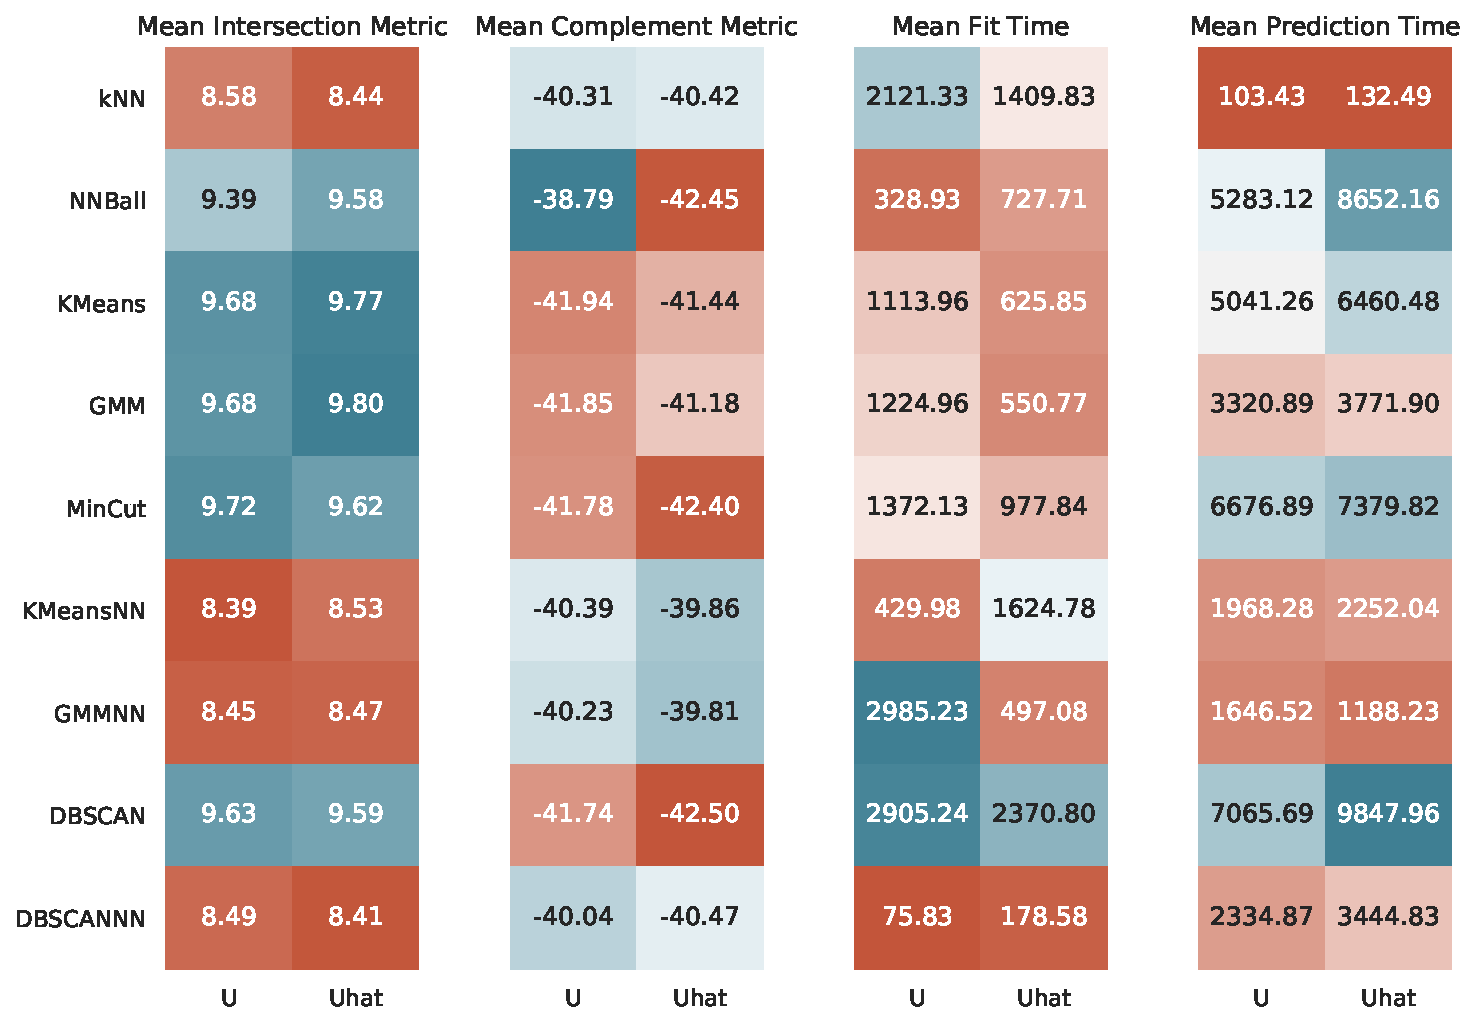
\includegraphics[width=1\textwidth]{figs/user_rdr.pdf}
\caption{Comparison of Collaboration-Based Recommendation Algorithms}
\label{fig:user_rdr}
\end{figure}

\begin{figure}[t]
\centering
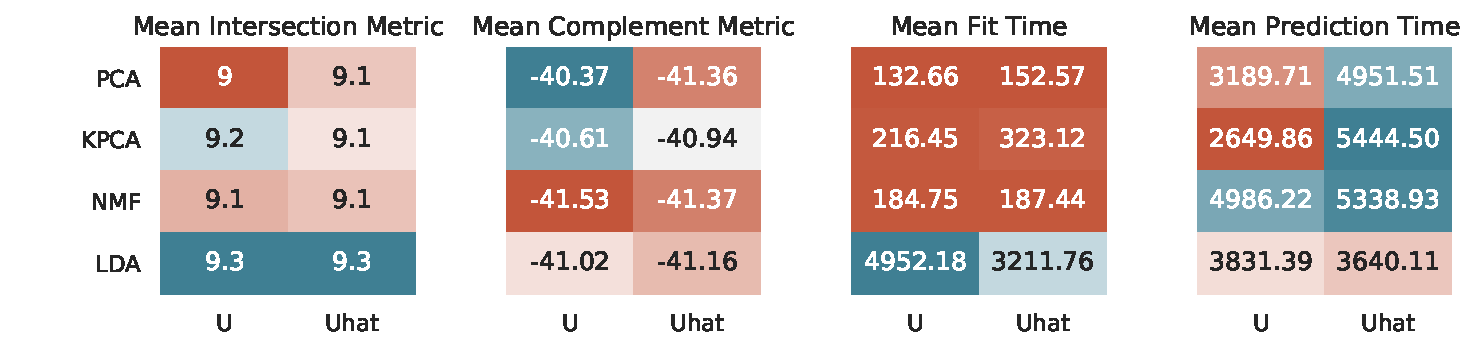
\includegraphics[width=1\textwidth]{figs/user_dr.pdf}
\caption{Comparison of Collaboration-Based Dimension Reduction Algorithms}
\label{fig:user_dr}
\end{figure}

\begin{figure}[t]
\centering
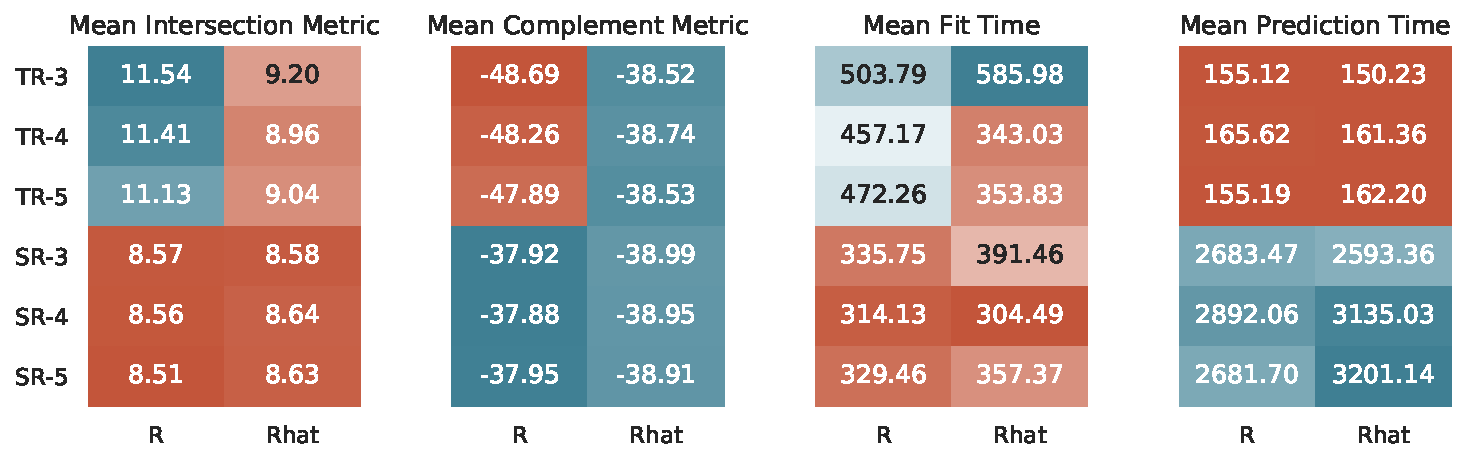
\includegraphics[width=1\textwidth]{figs/recipe_rdr.pdf}
\caption{Comparison of Content-Based Recommendation Algorithms}
\label{fig:recipe_rdr}
\end{figure}

\begin{figure}[t]
\centering
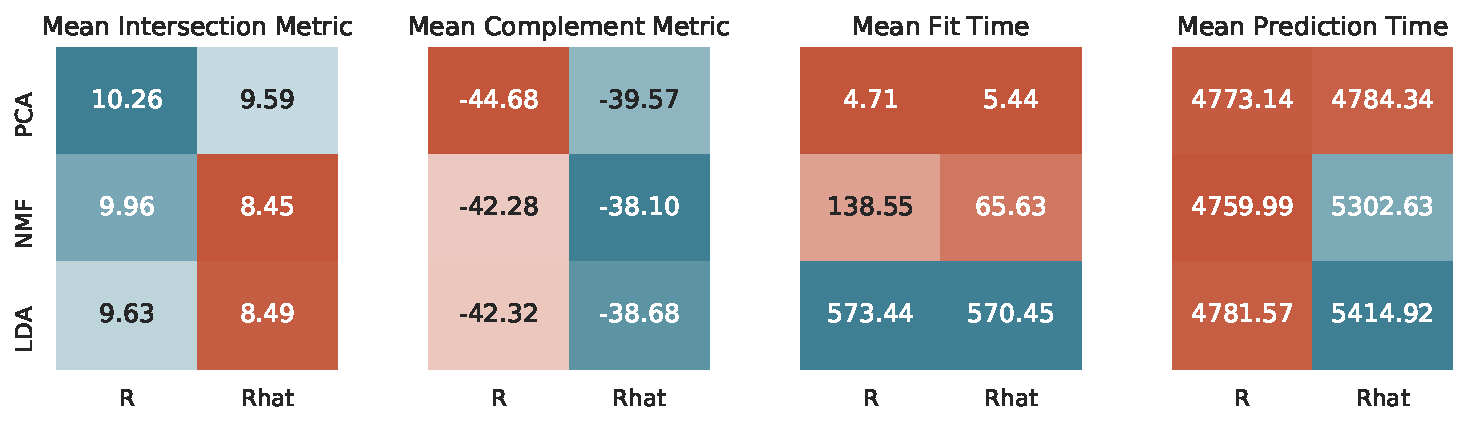
\includegraphics[width=1\textwidth]{figs/recipe_dr.pdf}
\caption{Comparison of Content-Based Dimension Reduction Algorithms}
\label{fig:recipe_dr}
\end{figure}


\section{Analysis}

\section{Conclusion}

\bibliographystyle{plain}
\bibliography{references}
\end{document}
